%---------- Inleiding ---------------------------------------------------------

% TODO: Is dit voorstel gebaseerd op een paper van Research Methods die je
% vorig jaar hebt ingediend? Heb je daarbij eventueel samengewerkt met een
% andere student?
% Zo ja, haal dan de tekst hieronder uit commentaar en pas aan.

%\paragraph{Opmerking}

% Dit voorstel is gebaseerd op het onderzoeksvoorstel dat werd geschreven in het
% kader van het vak Research Methods dat ik (vorig/dit) academiejaar heb
% uitgewerkt (met medestudent VOORNAAM NAAM als mede-auteur).
% 

\section{Inleiding}%
\label{sec:inleiding}

\subsection{Probleemstelling}

In de zorgindustrie wordt er steeds meer gesproken over 'alarmmoeheid'. Volgens \textcite{Ferrara2023} kan alarmmoeheid worden omschreven als ''een overprikkeling of zintuiglijke overbelasting, in staat tot het veroorzaken van gevoelloosheid ten opzichte van alarmen door een te groot aantal alarmen die foutief of klinisch onbelangrijk zijn.'' De ernst van de gevolgen van deze moeheid is echter verontrustend. Zo stelt \textcite{Ferrara2023} dat de gedragsmatige reactie van het verplegend personeel, dat lijdt aan een hoge alarmmoeheid, ongepast is. Deze reacties variëren tussen het geluid van het alarmsignaal aanpassen en volledige uitschakeling van het alarm. Wat dus een mogelijk gevaar voor de patiënt inhoudt. Deze stelling wordt bevestigd door het onderzoek van \textcite{Casey2018}. Uit hun onderzoek kwam naar voren dat 90,2 \%, van het geïnterviewde verplegend personeel, oordeelt dat foutieve of klinisch onbelangrijke alarmen frequent voorkomen, de patiëntenzorg verstoren en het vertrouwen in het alarmsysteem beschadigen. Verder zou tot 80,5\%, van het geïnterviewde verplegend personeel, het alarmsysteem soms deactiveren.
\\\\
Twee van de onderdelen van dit alarm-/\\monitoringsysteem zijn het DECT-systeem en het BELET-systeem. Het DECT-systeem is het audiosysteem dat gebruikmaakt van een mobiel toestel om binnen een bedrijf, in deze situatie een ziekenhuis, tussen diensten en personeel te communiceren. Hoewel het systeem al een hele tijd bestaat, sinds 1993, toch zijn er enkele gebreken. Zo is er interferentie met andere medische apparatuur, bedekkingsbeperkingen en de gelimiteerde functionaliteit. De laatste zou een update/upgrade kunnen gebruiken om visuele ondersteuning te bieden aan het personeel.
In tegenstelling tot het DECT-systeem, ligt het BELET-systeem volledig bij de patiënt. Deze is in bezit van een alarmknop waarmee hulp kan worden opgeroepen. Deze alarmsignalen kunnen ook foutief zijn, en zo bijdragen aan de alarmmoeheid.\\

Volgens \textcite{Coiera2006} bestaat de informatie-uitwisseling in gezondheidszorg voornamelijk uit communicatie tussen personen. Dit wordt een ''Communication space'' genoemd. Dit omvat onder andere conversaties over telefoon en in persoon, e-mails, brieven, \ldots . Verder wijst het onderzoek van \textcite{Coiera2006} aan dat de complexiteit van conversaties stijgt naarmate er meer mensen betrokken raken. Dit komt omdat er verschillende conversaties tussen 2 personen kunnen gevoerd worden.

\begin{figure}[h]
  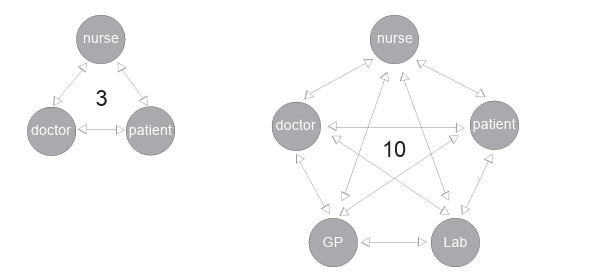
\includegraphics[width=\linewidth]{../graphics/Number-of-conversations.png}
  \caption{Aantal mogelijke conversaties stijgt samen met het aantal personen dat deelneemt aan communicatie. Uit ''Communication Systems in Healthcare'' door \autocite{Coiera2006}}
  \label{fig:aantal conversaties}
\end{figure}

Het is de combinatie van de stijging in complexiteit van informatie uitwisselen met de nadelen van het DECT-systeem en de gevaren van alarmmoeheid die ervoor zorgen dat het huidige systeem wordt in vraag getrokken. Zo bekomen we ook de hoofdvraag die wordt behandeld in deze bachelorproef: \textit{''Hoe kunnen technologieën worden ingezet om de communicatie aan te pakken in de gezondheidszorg?''}.\\

Om op deze vraag te antwoorden zullen er verschillende deelvragen moeten worden beantwoord:
\begin{enumerate}
  \item \textit{Wat zijn de kenmerken van het DECT-\\systeem?}
  \item \textit{Wat is het huidige systeem (met \hyphenation{rand-apparatuur}randapparatuur) en wat zijn de nadelen hiervan?}
  \item \textit{Hoe kan een zorgsituatie worden gesimuleerd?}
\end{enumerate}

\subsection{Bachelorproef}
Deze bachelorproef zal focussen op het onderzoeken van welke innovaties een waardevol alternatief kunnen zijn voor het DECT-systeem. Dit onderzoek is gericht op IT-personeel in gezondheidszorginstituten.\\\\

Om een antwoord te formuleren op de hoofdvraag zullen er tussenstappen worden genomen. Deze tussenstappen zijn opgesteld als deelvragen:

\begin{enumerate}
  \item \textit{Welke pogingen zijn al ondernomen om het DECT-systeem als standaard?}
  \item \textit{Wat zijn de minimumvereisten voor technologieën, om als alternatief te kunnen \\worden beschouwd?}
  \item \textit{Welke andere communicatiemogelijkheden zijn er die voldoen aan de minimumvereisten?}
  \item \textit{Welke mogelijke data-integratiemogelijkheden hebben de alternatieven?}
  \item \textit{Welke eigenschappen van het alternatief hebben een vermindering in alarmmoeheid als gevolg?}
  \item \textit{Vanaf wanneer is het haalbaar om te implementeren op economisch vlak?}
\end{enumerate}

De proof of concept die wordt opgesteld tijdens de bachelorproef is in samenwerking met Citymesh en met 360° Zorglab. Citymesh is een bedrijf dat zich specialiseert in connectiviteit, met focus op permanente en tijdelijke netwerkinfrastructuur. Dit door gebruik te maken van WiFi, 0G-, 4G- en 5G-technologieën. \autocite{Citymesh2024} Het 360° Zorglab is een project van HOGENT. De kern van het Zorglab is het creëren van een wisselwerking tussen disciplines enerzijds en tussen onderzoek, dienstverlening en onderwijs anderzijds. Toekomstige gezondheids- en welzijnsmedewerkers kunnen hier in een veilige omgeving niet-technische skills aanleren in een interprofessionele context. \autocite{HOGENT2024} Het doel van deze samenwerking is een snelle wisselwerking te kunnen creëren om zo meerdere malen de testfases te kunnen doorlopen. 

%---------- Stand van zaken ---------------------------------------------------
\section{Literatuurstudie}%
\label{sec:literatuurstudie}

De huidige stand van zaken kan worden opgedeeld in 4 delen. Het eerste deel is een situatieschets van de huidige complete set-up, met al zijn gebreken en voordelen. Vervolgens is er een oplijsting van mogelijke alternatieven, gevolgd door de minimumvereisten voor een communicatiesysteem ter vervanging van het DECT-systeem. Na de oplijsting van de alternatieven en vereisten worden de alternatieven onder de loep genomen om hun eigenschappen en mogelijke gebruikswijzen aan te tonen. Als derde deel wordt er gekeken naar de mogelijke gebruik van data. Tenslotte is er de wetgeving en de veiligheidsaspecten die gepaard gaan met een communicatiesysteem voor gezondheidszorg.

\subsection{DECT-systeem}
Het DECT-systeem staat voor Digital Enhanced Cordless Telecommunications; dit is een standaard in de EU sinds 1993. De meest gebruikte situatie is waar er meerdere gebruikers zijn voor een draadloze communicatie in werkomgevingen. De voornaamste reden voor gebruik van het DECT-\\draadloos systeem is dat het een grote dichtheid van veel gebruikers aankan. In vergelijking met andere mobiele communicatiesystemen werkt het niet buiten de werkomgeving. \autocite{Welinder1997} Na onderzoek van \textcite{Welinder1997} bleek dat de interferentie van het DECT-systeem op medisch gereedschap 11 procent was. De interferentie valt echter volledig weg bij een afstand van 0,5m tussen het gereedschap en het DECT-toestel.


Hoewel het DECT-systeem een standaard is sinds 1993, zijn er toch verschillende innovaties toegepast op dit systeem, maar deze worden als een apart systeem gezien. 

\subsection{Andere communicatietechnologieën}

Door studies van \textcite{Montalvo2024}, \textcite{Kranz2010} en \textcite{Soenmez2018} kan er een lijst worden opgesteld van alternatieven voor het DECT-systeem:

\begin{itemize}
  \item LTE Advanced
  \item 5G
  \item ULE
  \item VoIP

\end{itemize}

\subsubsection{Minimumvereisten}

Volgens \textcite{Coiera2006} zijn de volgende zaken vereist om te spreken van een communicatiesysteem:
\begin{itemize}
  \item Communicatiekanaal
  \item Boodschap
  \item Communicatiebeleid
  \item Communicatie toestel
  \item Interacties
  \item Beveiligingsbeleid
\end{itemize}

Verder zijn er eisen omwille van het gebruik van dit communicatiesysteem in de gezondheidszorg:

\begin{itemize}
  \item Wetgeving conform (EHDS, NIS2, GDPR, \dots)
  \item Gesloten systeem
  \item Interne data gebruik mogelijk
  \item Opties voor meer dan enkel audiocommunicatie
  \item Stabiel
  \item Schaalbaar
  \item Filter-functionaliteit mogelijk
\end{itemize}

Het is belangrijk ook om te vermelden dat in deze bachelorproef enkel Inter-ziekenhuis communicatie wordt onderzocht. Dit betekent dat enkel binnen eenzelfde site wordt gekeken om een oplossing of alternatief te bieden voor het DECT-systeem.

\subsubsection{LTE Advanced}

LTE of Long Term Evolution is de overkoepelende technologie waaronder 5G valt. Volgens \textcite{Bakare2022} is ook een verbetering van LTE Advanced, een stap naar de toekomst van LTE. De voornaamste eigenschappen van LTE Advanced zijn, opgelijst door \textcite{Bakare2022}:

\begin{itemize}
  \item Drie keer beter in spectrumefficiëntie in vergelijking met LTE
  \subitem 30 bps/Hz downlink
  \subitem 15 bps/Hz uplink
  \item Datapiek 
  \subitem 1 Gbps downlink
  \subitem 500 Mbps uplink
  \item Ondersteuning voor schaalbare bandbreedte en spectrumaggregatie
  \item Lage latentie
  \item Zeer goede compatibiliteit met LTE
\end{itemize}

\subsubsection{5G}
5G is een stap in de evolutie van het mobiele netwerk, opvolger van 4G. In deze bachelorproef gaat het om het private 5G-netwerk. Volgens \textcite{wen2021private} zijn er eigenschappen van private 5G die nauw aansluiten met die van DECT-systemen. De eerste eigenschap wijst op de hoge apparatuurdichtheid, maar bij 5G gaat deze ook nog eens gepaard met hoge throughput. Dit zorgt voor integratie van externe devices, zoals sensoren, camera's, etc. Vervolgens heeft 5G ook voordelen ten opzichte van DECT-systemen volgens \textcite{wen2021private}. Zo is er een hoge betrouwbaarheid met een lage latency. Deze lage latency geeft nieuwe mogelijkheden, zoals bv. een chirurgische ingreep vanop afstand.\\ De tweede eigenschap van het privaat netwerk is de flexibiliteit en voorspelbaarheid van Quality of Service (QoS). Daarnaast zijn er verschillende architecturen die men kan implementeren om een privaat 5G-netwerk op te zetten. De eerste methode is een stand-alone deployment. Hierbij wordt een privaat netwerk opgezet, waarbij alle netwerk functies van het netwerk zijn gelimiteerd binnen een logische perimeter bestaande uit vooraf gedefinieerde regio's. De andere methode is een publiek netwerk geïntegreerd deployment. Deze architectuur kan worden opgesplitst in verschillende types, afhankelijk van de gradatie van integratie. Deze 4 types zijn de volgende:

\begin{itemize}
  \item O-RAN (Open Radio Access Network)
  \item Gedeelde RAN (Radio Access Network)
  \item Gedeelde RAN en controle vlak
  \item Gehost bij het Publieke Netwerk
\end{itemize}

\textcite{wen2021private} vermeldt ook dat er naast architectuur een keuze moet worden gemaakt voor het spectrum. Hier zijn ook opnieuw 3 keuzes: een dedicated privaat spectrum, een erkend spectrum en een niet-erkend spectrum. 
5G heeft een aantal noodzakelijke technologieën nodig in het netwerk. Een van deze technologieën is network slicing. Hierbij wordt er 'een netwerk in een netwerk' gemaakt door het fysieke netwerk op te splitsen in meerdere logische netwerken. Om aan network slicing te kunnen doen, is er een nood aan netwerkvirtualisatie. Het slicing zelf kan worden opgedeeld in 3 lagen: Infrastructuurlaag, Network-slice laag en Onderhoudslaag. De levensloop van het slicen van een netwerk verloopt volgens de volgende 4 fases \autocite{wen2021private}:

\begin{enumerate}
  \item Voorbereiding
  \item In dienst stellen
  \item Gebruik
  \item Ontmanteling
\end{enumerate}

\textbf{Connecties tussen 5G en gezondheidszorg}

Het derde luik van de literatuurstudie gaat dieper in op de connecties tussen 5G en gezondheidszorg, en hoe deze worden bereikt aan de hand van bestaande frameworks. Er zijn verschillende mogelijkheden, maar met de focus op een toegankelijke methode zal er voornamelijk gefocust worden op open-source frameworks. Zo lijst \textcite{Eswaran2022} de verschillende variaties op een open-source 5G-framework voor private 5G-netwerken op:

\begin{itemize}
  \item Magma
  \item 5G OpenRAN
  \item ONF's Aether platform
  \item ETSI OSM
  \item srsRAN
  \item OpenAirInterface UE
\end{itemize}

Volgens \textcite{Open5GS2024} is Open5G 'een geavanceerd open-source project ontworpen voor het bouwen en onderhouden van je eigen NR/LTE mobiele netwerk. Open5G biedt een robuuste oplossing voor het configureren van zowel 5G (NR) als LTE (Evolved) netwerken.' \\ Verder zijn er andere concepten zoals ORAN, waar onder andere het OpenCare5G-netwerk op gebaseerd is. In dit framework wordt Open RAN in een privaat netwerk gebruikt voor digitale gezondheidsapplicaties. Zo hebben \textcite{de2023opencare5g} onderzocht hoe dit framework kan gebruikt worden om gezondheidsonderzoeken te doen met draagbare ultrasone gereedschappen op verschillende locaties. Om deze onderzoeken te kunnen delen met artsen, werd er een lokaal privaat netwerk opgezet. Zo gebruikten ze een 5G xHaul ORAN Operations, Administration en Maintenance (OAM) privaat netwerk. Er wordt gekozen om een top-down systeem te gebruiken. Dit is een georganiseerde manier om een netwerk project te ontwikkelen. Dit komt doordat men kan steunen op het OSI-model en het 5G-RAN protocol layer model. Dit zal ook gebruikt worden bij de methodologie. Zo zal er een analyse zijn van elke laag van de 5G-architectuur. Deze architectuur begint met de service laag. Op deze laag komen de verzoeken van de applicatie vandaan. De architectuur eindigt met de infrastructuurlaag. \autocite{de2023opencare5g}

\subsubsection{ULE}

ULE is een uitbreiding op het DECT-systeem zelf. Volgens \textcite{GariniDil2014} is dit een samenwerking tussen het DECT-systeem, CAT-iq (nieuwste HD voice-technologie) en een nieuwste aanpassing van data technologie ULE (Ultra Low Energy). Aangezien dit een uitbreiding is op het huidige DECT-systeem is er dus een makkelijke installatie en compatibiliteit.

De grootste voordelen van deze technologie volgens \textcite{GariniDil2014} zijn:

\begin{itemize}
  \item Open wereldwijde standaard
  \item Interferentievrije frequentieband
  \item Verbeterde veilige range
  \subitem Alle communicatie is versleuteld
  \item Lage kost
  \item Video en audio
\end{itemize}

\subsubsection{VoIP}

VoIP of Voice Communication over the Internet Protocol is een communicatietechnologie dat telefooncommunicatie stuurt over het internet in plaats van het telefoonnetwerk te gebruiken. \Autocite{Soenmez2018} Er zijn 5 scenario's waarin VoIP kan worden gebruikt. Deze worden opgelijst door \textcite{Soenmez2018}:

\begin{itemize}
  \item Computer naar Computer
  \item Computer naar telefoon (PSTN) (of omgekeerd)
  \item Telefoon (PSTN) naar Telefoon (PSTN)
  \item Mobiele VoIP
  \item Draadloze VoIP
\end{itemize}

Echter, \textcite{Soenmez2018} bevestigt wel dat er een groot aanvalsoppervlak bestaat. Zo heeft de Voice Over IP Security Allliance (VOIPSA) een lijst gepubliceerd met 6 beveiligingspunten waar countermeasures moeten geinstalleerd worden om een veilige omgeving te garanderen.

\subsection{Data}

Volgens \textcite{Niekerk2020} is de gezondheidszorg rijk aan data en is deze data ook nog eens waardevol. Toch wordt er maar 50\% gebruikt 
De data kan een ondersteunende factor zijn om de alarmmoeheid weg te werken. Zo onderzocht \textcite{Hever2019} de mogelijkheid om met data en machine learning de valse alarmen te verminderen. In dat onderzoek werd dit getest op de Intensieve Zorg afdeling. In de conclusie van \textcite{Hever2019} stelt deze dat door het gebruik van deze data er een AI-model opgeleid kon worden om de afdeling stiller en betrouwbaarder te maken. Dit verminderde het effect van alarmmoeheid. Verder meldt \textcite{Hever2019} dat door deze data en het model  ontbrekende factoren kunnen interpoleren.


\subsection{Security}
In samenspraak met de co-promotor is er geopteerd om cybersecurity niet actief te onderzoeken in deze bachelorproef. Echter, het is wel noodzakelijk om te weten dat er verschillende verplichtingen zijn in België en de Europese Unie. Als men een introductie van een 5G-netwerk uitvoert in een gezondheidszorgomgeving en/of ziekenhuizen is er sprake van een vergroting van de 'attack surface'. De beveiliging van dit type omgeving, ook wel de beveiliging van gezondheidszorg 5.0 genoemd, doet een beroep op de CIA-principes. Echter, \textcite{Wazid2022} voegt nog enkele extra eisen toe:

\begin{itemize}
  \item Beschikbaarheid
  \item Integriteit
  \item Vertrouwelijkheid
  \item Toegangscontrole
  \item Beschikbaarheid
  \item Voorwaartse geheimhouding
  \item Achterwaartse geheimhouding
  \item Onweerlegbaarheid
\end{itemize}

Als al deze principes worden toegepast, kan men stellen dat er voldaan is aan de minimum noodzakelijke beveiliging van het gezondheidszorgsysteem. Zo stelt \textcite{Wazid2022} vier reeds bestaande schema's voorop voor de beveiliging van dit systeem, elk met hun taak, features en beperkingen:

\begin{itemize}
  \item B2H \autocite{Ghosh2022}
  \item Blockchain en quantum-blindhandtekening \autocite{Bhavin2021}
  \item Systeembreed sleutelschema \autocite{Chang2022}
  \item Blockchain-gedreven intelligent schema voor telechirurgiesysteem (BITS) \autocite{Gupta2020}
\end{itemize}

\subsubsection{Wetgevingen}

Sinds 27 april 2016 is de verordening 2016/679 van toepassing. Deze start de GDPR (General Data Protection Regulation) in de Europese Unie. De verordening 2016/679 vermeldt dat "regels worden vastgelegd betreffende de bescherming van natuurlijke personen in verband met de verwerking van persoonsgegevens en het vrije verkeer van persoonsgegevens. Het beschermt de grondrechten en de fundamentele vrijheden van natuurlijke personen, met name hun recht op bescherming van persoonsgegeven."\\ (Verordening (EU) 2016/679 van het Europees Parlement en de Raad van 27 april 2016) %\autocite{gdpr2016} 
\\\\
Vervolgens is er ook het NIS2, een Belgische wet die bedrijven verplichtingen oplegt op het vlak van cybersecurity. "De wet van 26 april 2024 tot vaststelling van een kader voor de cyberbeveiliging van netwerk- en informatiesystemen van algemeen belang voor de openbare veiligheid (de "NIS2-wet") zet de EU-richtlijn 2022/2555 van het Europees Parlement en de Raad van 14 december 2022 (de "NIS2-richtlijn") om." \\
(Wet tot vaststelling van een kader voor de cyberbeveiliging van netwerk- en informatiesystemen van algemeen belang voor de openbare veiligheid van 26 april 2024) %\autocite{Belgium2024}
\\\\
Tenslotte is er een nieuwer initiatief genaamd EHDS (European Healthcare Data Space). Dit initiatief heeft het volgende doel: "De algemene doelstelling is te waarborgen dat natuurlijke personen in de EU in de praktijk meer zeggenschap over hun elektronische gezondheidsgegevens hebben."\\ (Voorstel (EU) COM/2022/197 van het Europees Parlement en de Raad van 3 mei 2022) %\autocite{EHDS2022}

% Voor literatuurverwijzingen zijn er twee belangrijke commando's:
% \autocite{KEY} => (Auteur, jaartal) Gebruik dit als de naam van de auteur
%   geen onderdeel is van de zin.
% \textcite{KEY} => Auteur (jaartal) Gebruik dit als de auteursnaam wel een
%   functie heeft in de zin (bv. ``Uit onderzoek door Doll & Hill (1954) bleek
%   ...'')

%---------- Methodologie ------------------------------------------------------

\section{Methodologie}%
\label{sec:methodologie}

% Alvorens de methodologie volledig wordt besproken; is er een belangrijke disclaimer noodzakelijk te vermelden.
% In samenspraak met de co-promotor is er geopteerd om cybersecurity niet actief te onderzoeken in deze bachelorproef thesis. Echter, het is wel noodzakelijk om te weten dat er verschillende verplichtingen zijn in België en de Europese Unie. In de literatuurstudie is er wel een kort naslagwerk van de verplichtingen ten opzichte van cybersecurity.
% \\\\

Tijdens het verloop van de bachelorproef zullen er antwoorden worden vergaard op verschillende deelvragen die helpen de onderzoeksvraag te beantwoorden. Zo zal elke deelvraag deel uitmaken van een onderdeel van de methodologie.
\\\\
De bachelorproef verloopt in de volgende fasen:

\begin{figure}[h]
  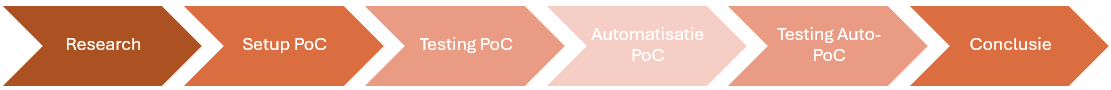
\includegraphics[width=\linewidth]{../graphics/Planning.png}
  \caption{Planning van de methodologie}
  \label{fig:Planning}
\end{figure}

\begin{enumerate}
  \item Research / Voorbereiding
  \item In dienst stellen / Setup
  \item Gebruik en testen
  \item Realisatiefactor bepaling
  \item Conclusie
\end{enumerate}

\subsection{Research / Voorbereidingsfase}
De eerste vraag die moet gesteld worden is: \textit{''Hoe kunnen technologieën worden ingezet om de communicatie aan te pakken in de gezondheidszorg?''}.\\ 

Hiermee wordt de onderzoeksfase gestart. De eerste stap van de onderzoeksfase is het in kaart brengen van het huidige DECT-systeem. Dit zal bekeken worden vanuit een algemeen overzicht. Het doel is om de werking en kenmerken van het DECT-systeem in kaart te brengen .\\
Vervolgens wordt er een opvolgvraag gesteld: \textit{''Wat is het huidige systeem (met \hyphenation{rand-apparatuur}randapparatuur) en wat zijn de nadelen hiervan?''} Hiermee wordt er diepgaand onderzoek gedaan naar het huidige systeem en zijn nadelen. Deze nadelen worden verzameld om achteraf deze te vergelijken het het alternatief.\\ Omdat deze bachelorproef in samenwerking is met 360° Zorglab, zal er onderzocht moeten worden \textit{''Hoe kan een zorgsimulatie worden gesimuleerd?''}. Als dit gekend is kan er een stappenplan worden opgesteld om het alternatief te kunnen testen in zo'n simulatie.
Nadat deze vragen te hebben beantwoord, is het probleem volledig in kaart gebracht.\\

% \item \textit{Welke pogingen zijn al ondernomen om het DECT-systeem als standaard te vervangen?}
% \item \textit{Wat zijn de minimum vereisten voor technologieën, om als alternatief te kunnen \\worden beschouwd?}
% \item \textit{Welke andere communicatie mogelijkheden zijn er die voldoen aan de minimum vereisten?}
% \item \textit{Welke mogelijke data-integratie mogelijkheden hebben de alternatieven?}


Zodra het probleem volledig is gekend, kan men aan de oplossing beginnen. Zo is het belangrijk om te weten: \textit{''Welke pogingen zijn al ondernomen om het DECT-systeem als standaard te vervangen?''} Dit kan inzicht geven in de mogelijke oplossingen. Verder kan men leren uit de tekortkomingenvan vorige pogingen. In combinatie met de vorige pogingen voor een standaardverandering is het noodzakelijk om testbare minimumvereisen te hebben of met andere woorden \textit{''Wat zijn de minimum vereisten voor technologieën, om als alternatief te kunnen worden beschouwd?''}. 
Eenmaal de minimum vereisten gekend zijn kunnen de opgelijste alternatieven onderworpen worden aan deze eisen. Als tussenstap in deze controle wordt elk alternatief ook getoetst op: \textit{''Welke mogelijke data-integratie mogelijkheden hebben de alternatieven?''}. Op deze manier is er een duidelijk antwoord op mogelijke verdere stappen na de bachelorproef voor automatisatie van foutanalyse of foutieve alarmen, met als doel de alarmmoeheid te verminderen en een betere zorg te kunnen bieden aan de patiënt.


% Deze vraag kan enkel beantwoord worden na een kort onderzoek in de verschillende frameworks, architecturen. Als besluit van dit onderzoek zal er een vergelijkende studie zijn. Hieruit wordt het best passende framework gekozen.
% Als vervolg op de keuze van het framework zullen de technische specificaties worden vastgelegd en opgelijst. Dit is een noodzakelijke stap om in de conclusie op het einde een duidelijk beeld te kunnen krijgen van mogelijke upsizing.\\
% De volgende deelvraag is: \textit{''Hoe kan een 5G-netwerk een oplossing bieden?''}.\\ Met deze vraag wordt er dieper onderzoek gedaan naar de huidige 5G-systemen/-frameworks. De laatste deelvraag van de research-/voorbereidingsfase is: \textit{''Hoe moet het 5G-netwerk eruitzien, rekening houdend met framework en scaling?''}\\ Hoewel dit de laatste stap is in de voorbereidende fase, is deze cruciaal voor alle verdere fases. Hier wordt alle informatie vergaard in de researchfase en in een netwerkschema/-topologie verwerkt. Dit zal als leidraad worden gebruikt in het verdere verloop van de bachelorproef.

\subsection{In dienst stellen / Setup-fase}
Deze fase bestaat uit het omzetten van de verworven theorie naar een proof-of-concept (PoC). Deze bachelorproef zal bestaan uit 2 PoC's. De eerste zal een simulatie zijn die lokaal op de pc werkt. Het tweede deel is een praktische realisatie, met de artikelen opgelijst in de technische specificaties.

\subsubsection{POC 1: Lokale testomgeving}
De testomgeving wordt opgesteld op de laptop van de student. Dit zal gebruikmaken van de volgende tools:

\begin{itemize}
  \item Vagrant
  \item Ansible
  \item VirtualBox
\end{itemize}

\subsubsection{POC2: Praktische realisatie}

Voor de praktische realisatie wordt er gebruikgemaakt van materiaal aangeleverd door Citymesh en 360° Zorglab. Dit materiaal zal in het zorglab blijven als een vaste opstelling. De noodzakelijke hardware wordt opgesplitst in categorieën:

\begin{itemize}
  \item Software Defined Radio (SDR)
  \item Antenna
  \item Simkaart(en)
  \item Mobiel toestel (5G-compatibel)
  \item Kleine server
\end{itemize}

Deze lijst zal meegroeien met het project.

\subsection{Gebruik en Testfase}
Het doel van deze fase is het gebruiken en testen van de opstelling. Dit is voor optimalisatie, maar ook voor aftoetsing of de minimumvereisten ook in de praktijk zijn bereikt. De gebruik- en testfase verloopt net zoals de setupfase in twee delen. Het eerste deel is het opstellen van een eenduidig en gedetailleerd testplan. Dit gebeurt voor elke PoC. Hierna volgt de uitvoering van deze testplannen op hun respectievelijke PoC. Het is belangrijk dat tijdens de testfase verschillende activiteiten correct worden uitgevoerd. Zo is het noodzakelijk om gedetailleerde notities te hebben in geval van problemen. Een tweede factor die hier nauw bij samenhangt, is de reproduceerbaarheid van de fout of het probleem. Vervolgens zijn de duur en intensiteit van de test belangrijk. Daarom worden de testplannen meerdere malen doorlopen met een vergrotende tijdsduur en belasting- of gebruikintensiteit. Dit alles wordt ook opgenomen in een testverslag dat in de conclusiefase wordt verwerkt. In dit verslag wordt er ook een antwoord geformuleerd op de vraag: \textit{''Hoe kan de proof of concept voor de simulatie worden aangepast om in realiteit te kunnen gebruiken?''}. Dit zal een onderdeel zijn van de conclusie van het testverslag. Als laatste stap wordt een antwoord geformuleerd op de vraag: \textit{''Welke eigenschappen van het alternatief hebben een vermindering in alarmmoeheid als gevolg?''}.

\subsection{Realisatiefactor bepaling}
Deze fase is er om een antwoord te bieden op de vraag: \textit{''Vanaf wanneer is het haalbaar om te implementeren op economisch vlak?''}. Deze vraag komt vanuit Citymesh. Als antwoord hierop wordt er gekeken naar de gradatie van het netwerk en de voordelen ten opzichte van de kosten. Deze afweging wordt zowel gemaakt voor kleine als grote ziekenhuizen. Deze afweging wordt dan gebundeld om het kantelpunt te achterhalen. \\ Voor deze bepaling wordt er gebruikgemaakt van zowel installatiekost als onderhoudskosten, maar ook van de voordelen die nieuwere systemen hebben ten opzichte van het personeel en hun efficiëntie en effectiviteit. 


\subsection{Conclusie}
In de conclusie is er maar één doel. Dit is de onderzoeksvraag beantwoorden: \textit{''Hoe kunnen technologieën worden ingezet om de communicatie aan te pakken in de gezondheidszorg?''} In deze fase wordt alles uit vorige fases verzameld en verwerkt tot een concreet antwoord en een conclusie op deze vraag. Het eindresultaat zal de bachelorproef zijn. Tenslotte wordt er een korte vergelijking gemaakt van het DECT-systeem met de PoC.
\\\\
Doorheen de hele bachelorproef wordt verwacht dat er een open en directe communicatie is tussen de student en de co-promotoren. Dit is belangrijk omwille van het einddoel van de bachelorproef. Hoewel de onderzoeksvraag een antwoord wil op mogelijke vervanging/integratie, is het de bedoeling dat de tweede PoC in gebruik kan worden genomen door de Hogeschool Gent Departement Gezondheidszorg. Met als doel om een simulatie te kunnen bieden aan de studenten van een vervangoptie van het DECT-systeem, om alarmmoeheid tegen te gaan.

%---------- Verwachte resultaten ----------------------------------------------

\section{Verwacht resultaat, conclusie}%
\label{sec:verwachte_resultaten}

Het doel van deze thesis is om een alternatief te bieden voor het verouderde DECT-systeem. Dit door eerst het DECT-systeem in kaart te brengen met zijn voordelen en nadelen, maar ook de gebreken en mogelijke problemen. Als eenmaal de gebreken gekend zijn, kan er gekeken worden om deze op te vangen met een moderner systeem zoals 5G. Er zijn echter verschillende alternatieven. Een zeer aanneembare verwachting is dat er zal worden gekozen voor een 5G privaat netwerk, omwille van zijn eigenschappen en de afweging tussen de voor- en nadelen. Hoewel er geen officiële standaard is voor 5G-netwerken binnen de gezondheidszorg, zal er een zo objectief mogelijke keuze worden gemaakt met een vergelijking tussen alle mogelijkheden. Een disclaimer is wel noodzakelijk, aangezien het hier gaat om een bachelorproef zal er voornamelijk gekeken worden naar open-source projecten, omwille van budgetten. \\\\
De Proof-of-Concept zal een simulatie zijn van een kleinschalig, privaat 5G-netwerk. Hoewel kleinschalig, zal het ontworpen zijn met het oog op schaalbaarheid. Het is te verwachten dat de 5G-oplossing een efficiëntere en accuratere manier voor communicatie zal zijn ten opzichte van het DECT-systeem. Verder wordt er een daling verwacht in het voorkomen van alarmmoeheid. Dit komt doordat er verschillende alarmsignalen gebundeld zullen worden. Er zal ook de mogelijkheid zijn om afbeeldingen of berichten te kunnen sturen, waardoor de arts de situatie van de patiënt beter kan inschatten.\\\\
Op de vraag vanuit Citymesh voor een techno-economische studie, wordt verwacht dat de kost voor het installeren en uitrollen van het private 5G-netwerk hoog zal zijn in vergelijking met het huidige DECT-systeem. Er zal een afweging moeten worden gemaakt ten opzichte van de kost en de mogelijke winst op lange termijn door welzijn van personeel en daling van incidenten, die te wijten zijn aan alarmmoeheid.\\\\
De volgende stap na deze bachelorproef is de mogelijke integratie van het systeem in de opleidingen binnen het departement Gezondheidszorg van HOGENT, om de studenten een alternatief te kunnen aanbieden ten opzichte van het DECT-systeem.